\documentclass[]{book}
\usepackage{lmodern}
\usepackage{amssymb,amsmath}
\usepackage{ifxetex,ifluatex}
\usepackage{fixltx2e} % provides \textsubscript
\ifnum 0\ifxetex 1\fi\ifluatex 1\fi=0 % if pdftex
  \usepackage[T1]{fontenc}
  \usepackage[utf8]{inputenc}
\else % if luatex or xelatex
  \ifxetex
    \usepackage{mathspec}
  \else
    \usepackage{fontspec}
  \fi
  \defaultfontfeatures{Ligatures=TeX,Scale=MatchLowercase}
\fi
% use upquote if available, for straight quotes in verbatim environments
\IfFileExists{upquote.sty}{\usepackage{upquote}}{}
% use microtype if available
\IfFileExists{microtype.sty}{%
\usepackage{microtype}
\UseMicrotypeSet[protrusion]{basicmath} % disable protrusion for tt fonts
}{}
\usepackage[margin=1in]{geometry}
\usepackage{hyperref}
\hypersetup{unicode=true,
            pdftitle={GAMA Model Documentation},
            pdfauthor={Srirama Bhamidipati, Erika S, Arend L},
            pdfborder={0 0 0},
            breaklinks=true}
\urlstyle{same}  % don't use monospace font for urls
\usepackage{natbib}
\bibliographystyle{plainnat}
\usepackage{color}
\usepackage{fancyvrb}
\newcommand{\VerbBar}{|}
\newcommand{\VERB}{\Verb[commandchars=\\\{\}]}
\DefineVerbatimEnvironment{Highlighting}{Verbatim}{commandchars=\\\{\}}
% Add ',fontsize=\small' for more characters per line
\usepackage{framed}
\definecolor{shadecolor}{RGB}{248,248,248}
\newenvironment{Shaded}{\begin{snugshade}}{\end{snugshade}}
\newcommand{\AlertTok}[1]{\textcolor[rgb]{0.94,0.16,0.16}{#1}}
\newcommand{\AnnotationTok}[1]{\textcolor[rgb]{0.56,0.35,0.01}{\textbf{\textit{#1}}}}
\newcommand{\AttributeTok}[1]{\textcolor[rgb]{0.77,0.63,0.00}{#1}}
\newcommand{\BaseNTok}[1]{\textcolor[rgb]{0.00,0.00,0.81}{#1}}
\newcommand{\BuiltInTok}[1]{#1}
\newcommand{\CharTok}[1]{\textcolor[rgb]{0.31,0.60,0.02}{#1}}
\newcommand{\CommentTok}[1]{\textcolor[rgb]{0.56,0.35,0.01}{\textit{#1}}}
\newcommand{\CommentVarTok}[1]{\textcolor[rgb]{0.56,0.35,0.01}{\textbf{\textit{#1}}}}
\newcommand{\ConstantTok}[1]{\textcolor[rgb]{0.00,0.00,0.00}{#1}}
\newcommand{\ControlFlowTok}[1]{\textcolor[rgb]{0.13,0.29,0.53}{\textbf{#1}}}
\newcommand{\DataTypeTok}[1]{\textcolor[rgb]{0.13,0.29,0.53}{#1}}
\newcommand{\DecValTok}[1]{\textcolor[rgb]{0.00,0.00,0.81}{#1}}
\newcommand{\DocumentationTok}[1]{\textcolor[rgb]{0.56,0.35,0.01}{\textbf{\textit{#1}}}}
\newcommand{\ErrorTok}[1]{\textcolor[rgb]{0.64,0.00,0.00}{\textbf{#1}}}
\newcommand{\ExtensionTok}[1]{#1}
\newcommand{\FloatTok}[1]{\textcolor[rgb]{0.00,0.00,0.81}{#1}}
\newcommand{\FunctionTok}[1]{\textcolor[rgb]{0.00,0.00,0.00}{#1}}
\newcommand{\ImportTok}[1]{#1}
\newcommand{\InformationTok}[1]{\textcolor[rgb]{0.56,0.35,0.01}{\textbf{\textit{#1}}}}
\newcommand{\KeywordTok}[1]{\textcolor[rgb]{0.13,0.29,0.53}{\textbf{#1}}}
\newcommand{\NormalTok}[1]{#1}
\newcommand{\OperatorTok}[1]{\textcolor[rgb]{0.81,0.36,0.00}{\textbf{#1}}}
\newcommand{\OtherTok}[1]{\textcolor[rgb]{0.56,0.35,0.01}{#1}}
\newcommand{\PreprocessorTok}[1]{\textcolor[rgb]{0.56,0.35,0.01}{\textit{#1}}}
\newcommand{\RegionMarkerTok}[1]{#1}
\newcommand{\SpecialCharTok}[1]{\textcolor[rgb]{0.00,0.00,0.00}{#1}}
\newcommand{\SpecialStringTok}[1]{\textcolor[rgb]{0.31,0.60,0.02}{#1}}
\newcommand{\StringTok}[1]{\textcolor[rgb]{0.31,0.60,0.02}{#1}}
\newcommand{\VariableTok}[1]{\textcolor[rgb]{0.00,0.00,0.00}{#1}}
\newcommand{\VerbatimStringTok}[1]{\textcolor[rgb]{0.31,0.60,0.02}{#1}}
\newcommand{\WarningTok}[1]{\textcolor[rgb]{0.56,0.35,0.01}{\textbf{\textit{#1}}}}
\usepackage{longtable,booktabs}
\usepackage{graphicx,grffile}
\makeatletter
\def\maxwidth{\ifdim\Gin@nat@width>\linewidth\linewidth\else\Gin@nat@width\fi}
\def\maxheight{\ifdim\Gin@nat@height>\textheight\textheight\else\Gin@nat@height\fi}
\makeatother
% Scale images if necessary, so that they will not overflow the page
% margins by default, and it is still possible to overwrite the defaults
% using explicit options in \includegraphics[width, height, ...]{}
\setkeys{Gin}{width=\maxwidth,height=\maxheight,keepaspectratio}
\IfFileExists{parskip.sty}{%
\usepackage{parskip}
}{% else
\setlength{\parindent}{0pt}
\setlength{\parskip}{6pt plus 2pt minus 1pt}
}
\setlength{\emergencystretch}{3em}  % prevent overfull lines
\providecommand{\tightlist}{%
  \setlength{\itemsep}{0pt}\setlength{\parskip}{0pt}}
\setcounter{secnumdepth}{5}
% Redefines (sub)paragraphs to behave more like sections
\ifx\paragraph\undefined\else
\let\oldparagraph\paragraph
\renewcommand{\paragraph}[1]{\oldparagraph{#1}\mbox{}}
\fi
\ifx\subparagraph\undefined\else
\let\oldsubparagraph\subparagraph
\renewcommand{\subparagraph}[1]{\oldsubparagraph{#1}\mbox{}}
\fi

%%% Use protect on footnotes to avoid problems with footnotes in titles
\let\rmarkdownfootnote\footnote%
\def\footnote{\protect\rmarkdownfootnote}

%%% Change title format to be more compact
\usepackage{titling}

% Create subtitle command for use in maketitle
\newcommand{\subtitle}[1]{
  \posttitle{
    \begin{center}\large#1\end{center}
    }
}

\setlength{\droptitle}{-2em}
  \title{GAMA Model Documentation}
  \pretitle{\vspace{\droptitle}\centering\huge}
  \posttitle{\par}
  \author{Srirama Bhamidipati, Erika S, Arend L}
  \preauthor{\centering\large\emph}
  \postauthor{\par}
  \predate{\centering\large\emph}
  \postdate{\par}
  \date{2018-04-12}

\usepackage{makeidx}
\makeindex

\usepackage{amsthm}
\newtheorem{theorem}{Theorem}[chapter]
\newtheorem{lemma}{Lemma}[chapter]
\theoremstyle{definition}
\newtheorem{definition}{Definition}[chapter]
\newtheorem{corollary}{Corollary}[chapter]
\newtheorem{proposition}{Proposition}[chapter]
\theoremstyle{definition}
\newtheorem{example}{Example}[chapter]
\theoremstyle{definition}
\newtheorem{exercise}{Exercise}[chapter]
\theoremstyle{remark}
\newtheorem*{remark}{Remark}
\newtheorem*{solution}{Solution}
\begin{document}
\maketitle

{
\setcounter{tocdepth}{1}
\tableofcontents
}
\hypertarget{background}{%
\chapter*{Background}\label{background}}
\addcontentsline{toc}{chapter}{Background}

It is expected that in 2030 about 5 billion people will live in cities
as compared to the 3.6 billion now. This massive growth challenges the
liveability of urban environments. Designing sustainable cities
attractive to tourists, industry and commercial organizations as well as
pleasant to live in, requires a thorough understanding of urban dynamics
and the role of individual and collective human decision- making within
this

\hypertarget{introduction}{%
\chapter{Introduction}\label{introduction}}

Cities like other complex adaptive systems commonly develop in an
open-ended and often unexpected way with neighborhoods and urban
populations in constant development. These urban dynamics exhibit many
wicked problems in which the issue at hand as well the potential
solutions are strongly dependent on the perspectives of the multitude of
stakeholders involved.

Conflicting use-patterns among city users impact a multitude of urban
quality indicators and result in specific spatial-temporal patterns and
conflicts (Fig. 1). Currently, our understanding of these complex
processes remains limited and even more so our capacity to anticipate
these complex developments.

\hypertarget{objective}{%
\section{Objective}\label{objective}}

Against this backgound the objective of the City Simulation Lab is:

\begin{enumerate}
\def\labelenumi{\arabic{enumi})}
\tightlist
\item
  To develop a City Simulator toolbox including various agent-based
  models of urban systems
\item
  To increase our current understanding of complex urban processes
  leading to specific spatial-temporal patterns through simulation of
  urban systems through the implementation of the agent-based simulation
  toolbox.
\item
  To improve the capacity to anticipate complex urban dynamics through
  interactive participatory workshops developing and implementing a
  Participatory Urban Modelling (PUM) framework.
\end{enumerate}

\hypertarget{methods}{%
\section{Methods}\label{methods}}

\hypertarget{case-tourism-expansion-in-amsterdam}{%
\subsection{Case: Tourism expansion in
Amsterdam}\label{case-tourism-expansion-in-amsterdam}}

Amsterdam has seen a steep 40\% increase in tourists in just five years,
with currently 17 million people visiting the city on annual basis. This
strong increase impacts the liveability of the city and causes conflicts
among different users of the city.

\hypertarget{participatory-urban-modelling-pum}{%
\subsection{Participatory Urban Modelling
(PUM)}\label{participatory-urban-modelling-pum}}

In order to include the different perspectives of local stakeholders, we
developed a Participatory Urban Modelling (PUM) framework. Within this
cyclic process researchers and stakeholders actively collaborate in the
development of the City Simulator toolbox through a combination of
(simulation) games (Fig.2). Through interactive gaming workshops,
stakeholders collectively define potential policy changes and explore
the impacts on quality indicators and spatial conflicts.

\begin{figure}
\centering
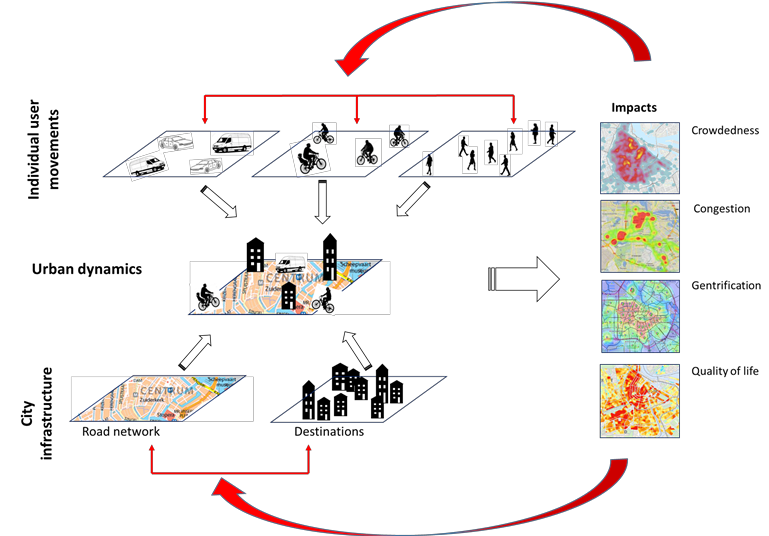
\includegraphics{images/scheme.png}
\caption{``PUM''}
\end{figure}

\hypertarget{imports}{%
\chapter{Imports}\label{imports}}

\hypertarget{species}{%
\chapter{Species}\label{species}}

The model has 4 species {[}inhabitants, buildings, roads, public
transport system{]}

\hypertarget{road}{%
\section{road}\label{road}}

This species is imported from a shapefile. The attributes of this
shapefile are imported and mapped into various model variables - as
attributes of the road species.

\begin{figure}
\centering
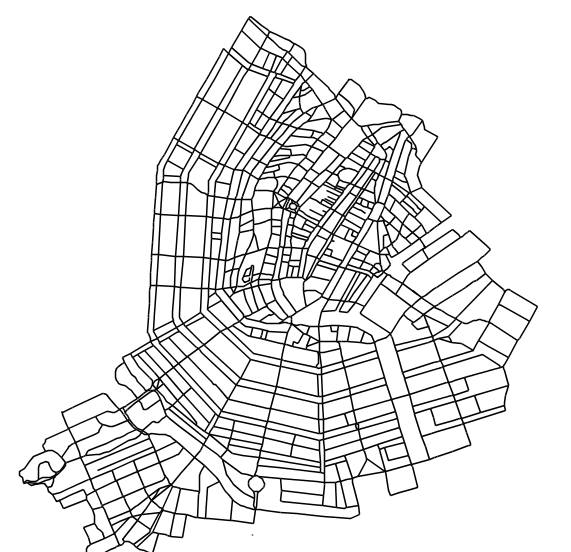
\includegraphics{images/network.png}
\caption{``Road Network''}
\end{figure}

\hypertarget{buildings}{%
\section{buildings}\label{buildings}}

This species is imported froma shapefile. The attributes of this
shapefile are imported and mapped into various model variables - as
attributes of the building species. The main classification of buildings
is based on its usage. Curerntly the model only distinguishes between
{[}office, home{]}.

\begin{figure}
\centering
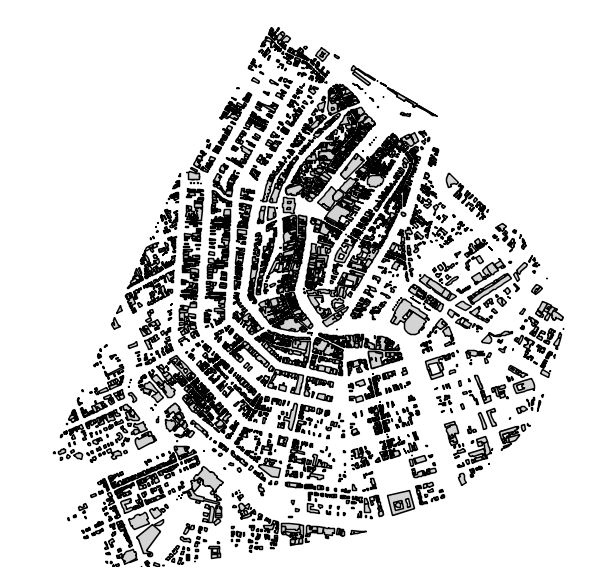
\includegraphics{images/buildings.png}
\caption{``Buildings''}
\end{figure}

\hypertarget{functions}{%
\chapter{Functions}\label{functions}}

\hypertarget{update_mode_specific_memory}{%
\section{update\_mode\_specific\_memory()}\label{update_mode_specific_memory}}

Agent memory on travel time is updated every day based on its experience
today. The agent uses last five days of memory to estimate the next days
travel time. This memory is mode specific. In this model, agent has 4
memories {[}walk, bike, pt, car{]}. \index{update! update memory}

\begin{Shaded}
\begin{Highlighting}[]
\NormalTok{action update_mode_specific_memory }\OtherTok{(}\KeywordTok{float}\NormalTok{ tt}\OtherTok{,} \KeywordTok{int}\NormalTok{ mode}\OtherTok{)}
\NormalTok{  \{}
        \CommentTok{//tt is morning_travel_time}
\NormalTok{        add tt to:self.mode_specific_memory}\OtherTok{[}\NormalTok{mode}\OtherTok{];}
\NormalTok{        remove index:}\DecValTok{0}\NormalTok{ from:self.mode_specific_memory}\OtherTok{[}\NormalTok{mode}\OtherTok{];}
        
\NormalTok{    \}}
\end{Highlighting}
\end{Shaded}

\hypertarget{arguments}{%
\subsection*{arguments}\label{arguments}}
\addcontentsline{toc}{subsection}{arguments}

\begin{itemize}
\tightlist
\item
  travel time (\texttt{float}) : the travel time experienced in the
  recent trip
\item
  mode (\texttt{int}) : the mode used by the agent in recent trip
\end{itemize}

\hypertarget{returns}{%
\subsection*{returns}\label{returns}}
\addcontentsline{toc}{subsection}{returns}

\begin{itemize}
\tightlist
\item
  nothing : the function returns nothing, it just updates an existing
  variable.
\end{itemize}

\hypertarget{usage}{%
\subsection*{usage}\label{usage}}
\addcontentsline{toc}{subsection}{usage}

\begin{itemize}
\tightlist
\item
  the following example updates memory of mode 1 = walk.
\end{itemize}

\begin{Shaded}
\begin{Highlighting}[]
\KeywordTok{do}\NormalTok{ update_mode_specific_memory}\OtherTok{(}\NormalTok{travel_time}\OtherTok{,} \DecValTok{1}\OtherTok{)}
\end{Highlighting}
\end{Shaded}

\hypertarget{evening_movement}{%
\section{evening\_movement()}\label{evening_movement}}

This function makes the agent move from office to home in the evening.
\index{movement! evening}

\begin{Shaded}
\begin{Highlighting}[]
\NormalTok{action evening_movement}
\NormalTok{    \{}
        \KeywordTok{float}\NormalTok{ my_speed <- mode_speed_int}\OtherTok{[}\NormalTok{self.value_mode_actual}\OtherTok{]} \OtherTok{;}\CommentTok{// # m / # sec;}
        \KeywordTok{do} \KeywordTok{goto}\NormalTok{ target: any_location_in}\OtherTok{(}\NormalTok{my_home}\OtherTok{)}\NormalTok{ on: g speed: my_speed}\OtherTok{;}
        \KeywordTok{if}\NormalTok{ the_target = location}
\NormalTok{        \{}
\NormalTok{            my_evening_home_arrive_time <- current_date}\OtherTok{;}
\NormalTok{        \}}

\NormalTok{    \}}
\end{Highlighting}
\end{Shaded}

\hypertarget{arguments-1}{%
\subsection*{arguments}\label{arguments-1}}
\addcontentsline{toc}{subsection}{arguments}

\begin{itemize}
\tightlist
\item
  none
\end{itemize}

\hypertarget{returns-1}{%
\subsection*{returns}\label{returns-1}}
\addcontentsline{toc}{subsection}{returns}

\begin{itemize}
\tightlist
\item
  nothing
\end{itemize}

\hypertarget{usage-1}{%
\subsection*{usage}\label{usage-1}}
\addcontentsline{toc}{subsection}{usage}

\begin{Shaded}
\begin{Highlighting}[]

\KeywordTok{do}\NormalTok{ evening_movement}\OtherTok{;}
\end{Highlighting}
\end{Shaded}

\hypertarget{morning_movement}{%
\section{morning\_movement()}\label{morning_movement}}

This function makes the agent move from office to home in the evening.
\index{movement! morning}

\begin{Shaded}
\begin{Highlighting}[]
\NormalTok{action evening_movement}
\NormalTok{    \{}
        \KeywordTok{float}\NormalTok{ my_speed <- mode_speed_int}\OtherTok{[}\NormalTok{self.value_mode_actual}\OtherTok{]} \OtherTok{;}\CommentTok{// # m / # sec;}
        \KeywordTok{do} \KeywordTok{goto}\NormalTok{ target: any_location_in}\OtherTok{(}\NormalTok{my_home}\OtherTok{)}\NormalTok{ on: g speed: my_speed}\OtherTok{;}
        \KeywordTok{if}\NormalTok{ the_target = location}
\NormalTok{        \{}
\NormalTok{            my_evening_home_arrive_time <- current_date}\OtherTok{;}
\NormalTok{        \}}

\NormalTok{    \}}
\end{Highlighting}
\end{Shaded}

\hypertarget{arguments-2}{%
\subsection*{arguments}\label{arguments-2}}
\addcontentsline{toc}{subsection}{arguments}

\begin{itemize}
\tightlist
\item
  none
\end{itemize}

\hypertarget{returns-2}{%
\subsection*{returns}\label{returns-2}}
\addcontentsline{toc}{subsection}{returns}

\begin{itemize}
\tightlist
\item
  nothing
\end{itemize}

\hypertarget{usage-2}{%
\subsection*{usage}\label{usage-2}}
\addcontentsline{toc}{subsection}{usage}

\begin{Shaded}
\begin{Highlighting}[]
\KeywordTok{do}\NormalTok{ morning_movement}\OtherTok{;}
\end{Highlighting}
\end{Shaded}

\hypertarget{reflexes}{%
\chapter{Reflexes}\label{reflexes}}

\hypertarget{displays}{%
\chapter{Displays}\label{displays}}

\hypertarget{experiment}{%
\chapter{Experiment}\label{experiment}}

\printindex


\end{document}
